\chapter{Evaluation}
This chapter details how the knowledge graph is evaluated upon completion and measures implementation success. Both qualitative and quantitative methods were used during this section to provide a comprehensive evaluation.

\section{Requirements-Based Assessment}
\hspace{0.5cm} Assessing whether the requirements listed in the \textit{Requirements} chapter were achieved is important to measure success of implementation. For each requirement, a description stating whether it was achieved will be provided. 

\subsection{Software Requirement Assessment}
\begin{longtable}{|p{2.25cm}|p{5.5cm}|p{5.5cm}|}

\hline
\textbf{Requirement No.} & \textbf{Software Requirement} & \textbf{Assessment}\\
\hline

1& 
Ontology must be correctly configured and input into SPARQL-Anything CONSTRUCT &
Ontology has been refined and adapted based on the needs of the project. All relationships or triples have either been derived from the provided ontology or appended to the ontology based on the dataset. \\
\hline

2&
The knowledge graph created must correctly reflect the organ dataset and follow ontology structure. &
Knowledge graph produced does reflect data from the organ dataset. More detail on the quality of the knowledge graph is in the next section. \\
\hline

3&
The dataset must be refined to ensure correct data is being input into the knowledge graph. &
Query correctly extracts the correct data from the dataset and adds it onto the knowledge graph. Data is usually mapped onto the ontology one-to-one, without further adjustment to ensure correct data is input into the knowledge graph. \\
\hline

4&
The knowledge graph must expand on the current dataset using external links. &
Using the organ Wikidata site \cite{organwikidata} and organ MusicBrainz site \cite{organmusicbrainz}, data was added to the existing knowledge graph. Custom links based on data in the dataset as well as other external links were also added as extensions to the knowledge graph. \\
\hline

5&
Knowledge graphs must be evaluated to prove correctness and validity. &
This will be evaluated in the next section: \textit{Knowledge Graph Assessment Quality} \\ 
\hline

6&
Scalability of knowledge graph generation must be assessed. &
This will be assessed and evaluated in detail in the \textit{Query Scalability Assessment} section. \\ 
\hline
\caption{Software Requirement Assessment Table}
\end{longtable}

\subsection{User Requirement Assessment}

\begin{longtable}{|p{2.25cm}|p{4.5cm}|p{6.5cm}|}
\hline
\textbf{Requirement No.} & \textbf{User Requirement} & \textbf{Assessment}\\
\hline

1& 
User must be able to execute written query. &
User can download SPARQL Anything \cite{sparqlanythinggithub} and execute a given query on command line. \\
\hline

2&
User must be able to select an organ to view information on. &
User can view the codes of all available organs in the dataset. This organ code can then be passed through command line, which generates a custom knowledge graph upon execution. \\
\hline

3&
User must be able to see the knowledge graph after the query is executed. &
User can either view the knowledge graph on command line or in a .TTL file with a specified location and file name. \\
\hline

4&
User must be able to see relevant data in the knowledge graph. &
User can view the knowledge graph and see relevant data corresponding to the requested organ. \\
\hline

5&
User must be able to view other relevant external data in the knowledge graph. &
User can view the knowledge graph and see external links as well as custom links based on data from the requested organ. \\ 
\hline

\caption{User Requirement Assessment Table}
\end{longtable}
\vspace{-1.1cm}

\section{Knowledge Graph Quality Assessment}
\hspace{0.5cm} Assessment of knowledge graph quality is important to ensure the produced knowledge graph is valid and correct, using \cite{knowledgegraphevaulationbook} as guidance to assess knowledge graph quality. The 18 qualitative requirements detailed in \cite{evaluationpaper} are also used to assess quality. For each section, specific details are assessed with explanations and assessment of knowledge graph quality. 

The main three sections used to assess knowledge graph quality are: 

\vspace{-0.2cm}
\begin{itemize}
    \itemsep0em 
    \item Accuracy
    \vspace{-0.15cm}
    \item Coverage
    \vspace{-0.15cm}
    \item Succinctness
\end{itemize}
\vspace{-0.1cm}

For each section, generated knowledge graphs for five different organs will be used to measure overall quality. Organs to be tested from the dataset are: \textit{Part14\_000Brouwershaven}, \textit{Part14\_000Niezijl}, \textit{Part14\_000Folsgare}, \textit{Part14\_000GravenhageNoorderkerk} and \textit{Part14\_000Groede}. For simplicity, a random sample of five was selected from the list of organ codes and the produced knowledge graphs will represent the quality of all possible organs. Generating the knowledge graphs and assessing quality from the output files was the method employed. 

\subsection{Accuracy}
\hspace{0.5cm} ``Accuracy refers to the extent to which entities and relations- encoded by nodes and edges in the graph- correctly represent real-life phenomena". \cite{knowledgegraphevaulationbook}. In this context, accuracy means the knowledge graph generated (both subjects and relationships) needs to correctly reflect the relationships between organ topics. 

There are three types of accuracy: 

\vspace{-0.2cm}
\begin{itemize}
    \itemsep0em 
\item Syntactic Accuracy.
\vspace{-0.1cm}
\item Semantic Accuracy.
\vspace{-0.1cm}
\item Timeliness.
\end{itemize}
\vspace{-0.4cm}

\subsubsection{Syntactic Accuracy}
\hspace{0.5cm} Syntactic accuracy refers to whether the data presented is valid for its given type. \cite{knowledgegraphevaulationbook}

\noindent An example of a potential violation: 
\begin{displayquote}
    \textit{``This is an organ" would be incompatible with xsd:integer.}
\end{displayquote}

Upon assessing the produced knowledge graphs for each of the five organs, no syntactic inaccuracies were found. Checks for each organ were carried out and due to the ontology being derived from the provided ontology and external links, all resulting knowledge graphs should not, in theory, contain any syntactic inaccuracies. 

\subsubsection{Semantic Accuracy}
\hspace{0.5cm} Semantic accuracy refers to whether data values are being correctly represented in a real-world context. \cite{knowledgegraphevaulationbook}

\noindent An example of a potential violation: 
\begin{displayquote}
    \textit{Date of build (for an organ) coming after today's date.}
\end{displayquote}

In regards to semantic accuracy, none of the five organs contained semantic inaccuracies upon assessment. This can be explained for similar reasons as above regarding the lack of syntactic inaccuracies. 

\subsubsection{Timeliness}
\hspace{0.5cm} Timeliness refers to how up-to-date or relevant the knowledge graph is with the real current state of the modern world \cite{knowledgegraphevaulationbook}. This is also in line with \cite{evaluationpaper} stating that ``Knowledge graphs should contain the latest resources to guarantee freshness".

\noindent An example of a potential violation:
\begin{displayquote}
    \textit{Organ's location stated as ``Netherlands", but has recently been moved to Portugal and the knowledge graph has not been updated.}
\end{displayquote}

In the produced knowledge graphs, violations of timeliness can occur due to the static nature of the dataset. An example of a violation may occur when the \textit{?divisionName} is no longer the organ's current disposition in real life, but data in the dataset is not up-to-date. This particular violation will occur over time as the organ's divisions can change over time. However, at the current moment in time, no timeliness violations occur in the five produced knowledge graphs.

\subsection{Coverage}
\hspace{0.5cm} ``Coverage refers to avoiding the omission of domain-relevant elements, which may yield incomplete results". \cite{knowledgegraphevaulationbook}. In this context, the knowledge graph must completely fill the ontology framework in all of its nodes and edges. This is to accurately represent the entire dataset given. 

\noindent There are two types of coverage: 

\vspace{-0.15cm}
\begin{itemize}
\itemsep0em 
\item Completeness.
\vspace{-0.1cm}
\item Representativeness.
\end{itemize}
\vspace{-0.4cm}

\subsubsection{Completeness}
\hspace{0.5cm} Completeness ensures the knowledge graph is correctly filled with all the relevant information present in a particular dataset. \cite{knowledgegraphevaulationbook}. Adding contextual information about entities and from different resources \cite{evaluationpaper} is also important to ensure completeness. 

\noindent Some examples of potential violations:

\vspace{-0.15cm}
\begin{displayquote}
    \textit{- Organ classes lacking information.}
\end{displayquote}
\vspace{-0.6cm}
\begin{displayquote}
    \textit{- Important values missing for a specific organ property.}
\end{displayquote}
\vspace{-0.1cm}

With regard to dataset coverage, most of the data is represented in the knowledge graph. Reasoning for the omission of some data is related to how it can be represented in the knowledge graph without it causing confusion. For example, the specific ranges of a given organ for each keyboard or pedal are omitted due to the possible confusion it may cause when representing the keyboard and pedal ranges (\textit{?range1} and \textit{?range2}). Also, representing all that data concisely would be challenging and it may be seen as unnecessary. However, this is only relevant to some data. 

Contextual information is added in the form of descriptions and custom links in all assessed knowledge graphs. The relationship \textit{oont:extraInformation}, for instance, provides context and extra detail for a specific node. 

Different resources can be seen in the five knowledge graphs such as: Wikidata links, data from the dataset and various other website links. 

\subsubsection{Representativeness}
\hspace{0.5cm} Representativeness ensures the knowledge graph does not involve any bias and does not exclude anything relevant. \cite{knowledgegraphevaulationbook}

\noindent Some examples of potential violations: 

\vspace{-0.1cm}
\begin{displayquote}
    \textit{- Under-represent organ data from other languages.}
\end{displayquote}  
\vspace{-0.6cm}
\begin{displayquote}
     \textit{- Under-represent people (e.g. organist, owner) from a particular gender, race etc. }  
\end{displayquote}
\vspace{-0.1cm}

Violations regarding under-representation stem from the dataset provided. For example, the dataset is written in Dutch so organ data is limited to the Dutch language. With regard to the under-representation of people, anyone involved with the organ is mentioned in all five knowledge graphs such as: \textit{?maintainer} and \textit{?builder} so no violations occur in that regard.

\subsection{Succinctness}
\hspace{0.5cm} ``Succinctness refers to the inclusion of relevant content that is represented in a concise and intelligible manner." \cite{knowledgegraphevaulationbook}. In this context, it means the knowledge graph created should be easily understandable and to the point. 

\noindent There are two types of succinctness: 

\vspace{-0.15cm}
\begin{itemize}
    \itemsep0em 
\item Representational Conciseness.
\vspace{-0.1cm}
\item Understandability.
\end{itemize}
\vspace{-0.4cm}

\subsubsection{Representational Conciseness}
\hspace{0.5cm} Representational conciseness refers to the extent in which the knowledge graph content is compactly represented \cite{knowledgegraphevaulationbook}. This is consistent with requirements from \cite{evaluationpaper} including: ``triples should be concise" and ``knowledge graph does not contain redundant triples".

\noindent An example of a potential violation: 
\vspace{-0.1cm}
\begin{displayquote}
    \textit{Containing two properties that serve the same purpose i.e.}
\end{displayquote}
\vspace{-0.5cm}
\begin{displayquote}
    \textit{- Organist}
\end{displayquote}
\vspace{-0.6cm}
\begin{displayquote}
    \textit{- Organ Player}
\end{displayquote}

\begin{figure}[H]
\begin{center}
    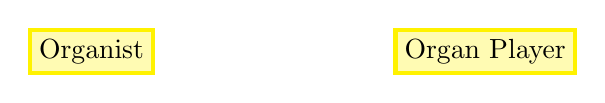
\begin{tikzpicture} [
        square/.style={draw=yellow, rectangle, ultra thick, fill=yellow!30},
        align=center,
        node distance=5cm ]
    \node[square] (q1)  {Organist};
    \node[square, right of=q1] (q2)  {Organ Player};
    \end{tikzpicture}
\end{center}
\vspace{-0.5cm}
\caption{Representational Conciseness Violation}
\end{figure}

Each knowledge graph is created with the purpose of making them concise. Creation of the ontology structure was derived and refined from the provided ontology. \textit{Figure 7.2} in the design was made specifically to represent the data in a concise manner and avoid the inclusion of redundant data. Implementation also kept this in mind when refining the ontology. Upon assessing each of the five organs, the produced knowledge graphs contain concise content.

\subsubsection{Understandability}
\hspace{0.5cm} Understandability refers to the need for readability and ease of understanding the knowledge graph generated. \cite{knowledgegraphevaulationbook}

\noindent An example of a potential violation: 
\vspace{-0.1cm}
\begin{displayquote}
    \textit{Using property names such as Organist1, when asked to state the name of an organist (Actual name should be used instead).}
\end{displayquote}

\begin{figure}[H]
\begin{center}
    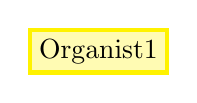
\begin{tikzpicture} [
        square/.style={draw=yellow, rectangle, ultra thick, fill=yellow!30},
        align=center,
        node distance=5cm ]
    \node[square] (q1)  {Organist1};
    \end{tikzpicture}
\end{center}
\vspace{-0.5cm}
\caption{Understandability Violation}
\end{figure}

Data in the dataset is understandable from the perspective of a Dutch reader. Given the relationships, the meaning of data can be easily inferred. However, there are some cases in the produced knowledge graphs where nodes produce an empty string ``" due to empty data in the dataset. For example, the variable \textit{?partition} in the ontology is often empty and out of the five tested organs, four of the \textit{partition}'s data is missing. 

From a lay user's perspective, it could also be argued that the Wikidata information can seem confusing at first glance due to the codes being displayed. However, this can be mitigated by physically clicking the URI link while viewing these external Wikidata links.  

\section{Query Scalability Assessment}
In this section, scalability of the knowledge graph will be tested. In particular, the areas being measured to assist quantification of the knowledge graph scalability are: 

\vspace{-0.1cm}
\begin{itemize}
\itemsep0cm
    \item Number of SERVICE Calls.
    \vspace{-0.1cm}
    \item Size of Files.
\end{itemize}
\vspace{-0.1cm}

For each one, measurement of scalability will be computed using the time required to execute the query on command line, which is how long it takes to generate the knowledge graph. This will make use of a command on the Windows OS called: \textit{Measure-Command} \cite{measurecommand}, which measures the time required for a command to execute. For instance, measuring the time required to generate a knowledge graph for organ: \textit{Part01\_001MIDDE} is:

\lstset
{
    breaklines=true,
    breakatwhitespace=false,
    basicstyle=\ttfamily,
}
\begin{lstlisting}
    Measure-Command{java -jar sparql-anything-0.8.1.jar -q queries/organ-details.sparql --values organ=Part01_001MIDDE -o output/output.ttl}
\end{lstlisting}

The same sample of five organs will be selected for knowledge graph generation and tests will be run on a 64-bit OS with Intel(R) Core(TM) i5-8265U CPU @ 1.60GHz 1.80 GHz and 8GB RAM. Regarding time calculation, the procedure will involve running each of the five sampled organs five times using \textit{Measure-Command}, followed by calculation of the average time per organ. Finally, the mean times for all five organs will be noted.

% knowledge of previous exponential, which is not a problem for our KG. but short term linear.
\subsection{Size of Files}
\hspace{0.5cm} For this test, knowledge graph generation was calculated with respect to .JSON file size (from the dataset). For testing purposes, some organs may be removed from relevant data files in order to measure the effect of file size. The five tested organs, however, will always remain in the files. This is possible since the structure of each .JSON file follows the same format as shown in the \textit{Context} section. External links were left in the query as their addition did not significantly affect results. After removing organs to test file size, the actual size of a file will be noted using a VS Code extension: \textit{filesize}. A graph plotted with cumulative file sizes against time can be seen in \textit{Figure 9.3}.

\begin{figure}[H]
\begin{center}
\begin{tikzpicture}
\begin{axis}[
    axis x line=bottom,
    axis y line=left,
    xlabel=\textit{file size (MiB)},
    ylabel=\textit{time (ms)}, ]
\addplot[smooth,blue] plot coordinates {
    (0.01,1353.7575)
    (7.498502, 1751.012)
    (11.9024, 2021.9029)
    (15.27645, 2213.0641)
    (21.8746, 2464.1894)
};
\end{axis}
\end{tikzpicture}
\end{center}
\vspace{-0.75cm}
\caption{Analysis of File Size}
\end{figure}

\textit{Figure 9.3} shows an initial linear relationship between the file size and time. This shows that the knowledge graph-generating query produced is scalable to a certain extent. It is unknown, however, how well the query will perform for much larger file sizes. 

\subsection{Number of SERVICE Calls}
\hspace{0.5cm} In this test, number of SERVICE calls within the query are tested to observe their effect on the speed of knowledge graph generation. In the implemented query, removal of SERVICE calls will be done incrementally and plotted against execution time. Measuring the number of SERVICE calls will indicate the scalability of the knowledge graph, providing insight into its capacity for expansion.

For this project, knowledge graph size will increase proportionally with the number of SERVICE calls. A mock knowledge graph was created using additional SERVICE calls that were not in the project scope and added for testing purposes to measure expandability. Data gathered from the SERVICE call was added to the mock knowledge graph. This was to account for the time taken to add data onto the knowledge graph during command execution. In this particular test, all external links in the knowledge graph were removed so as to not affect execution time. The plotted graph for number of SERVICE calls against time can be seen in \textit{Figure 9.4}.

\begin{figure}[H]
\begin{center}
\begin{tikzpicture}
\begin{axis}[
    axis x line=bottom,
    axis y line=left,
    xlabel=\textit{no. SERVICE calls},
    ylabel=\textit{time (ms)}, 
    ]
\addplot[smooth,blue] plot coordinates {
    (1, 1184.163)
    (10, 1318.7934)
    (20, 1730.7290)
    (29, 1975.1539)
    (39, 2143.491)
    (49, 2340.4259)
    (59, 2520.7234)
    (99, 3420.7116)
};
\end{axis}
\end{tikzpicture}
\end{center}
\vspace{-0.75cm}
\caption{Analysis of SERVICE Calls}
\end{figure}

After plotting the graph (\textit{Figure 9.4}) of up to 100 SERVICE calls, an initial linear relationship can be seen between variables. The expandability of the knowledge graph is possible within reason. However, this graph only plots values for up to 100 SERVICE calls so time required for extremely large amounts of SERVICE calls may differ. 
